\chapter{Conditional Probability}\label{chap:cond_prob} %\label{cond_prob_sec}

\begin{editingnotes}
\TBA{Short intro}
\end{editingnotes}

\section{Monty Hall Confusion}\label{sec:confuse_Monty}
Remember how we said that the Monty Hall problem confused even
professional mathematicians?  Based on the work we did with tree
diagrams, this may seem surprising---the conclusion we reached
followed routinely and logically.  How could this problem be so
confusing to so many people?

Well, one flawed argument goes as follows: let's say the contestant
picks door A.  And suppose that Carol, Monty's assistant, opens door B
and shows us a goat.  Let's use the tree diagram~\ref{fig:14A3} from
Chapter~\ref{probability_chap} to capture this situation.  There are
exactly three outcomes where contestant chooses door $A$, and there is
a goat behind door $B$:
\begin{equation}\label{aabaaccab}
(A, A, B),\ (A, A, C),\ (C, A, B).
\end{equation}
These outcomes have respective probabilities 1/18, 1/18, 1/9.

Among those outcomes, switching doors wins only on the last outcome
$(C, A, B)$.  The other two outcomes \emph{together} have the
\emph{same} 1/9 probability as the last one So in this situation, the
probability that we win by switching is the \emph{same} as the
probability that we lose.  In other words, in this situation,
switching isn't any better than sticking!

Something has gone wrong here, since we know that the actual
probability of winning by switching in 2/3.  The mistaken conclusion
that sticking or switching are equally good strategies comes from a
common blunder in reasoning about how probabilities change given some
information about what happened.  We have asked for the probability
that one event, [win by switching], happens, \emph{given} that another
event, [pick A $\QAND$ goat at B], happens.  We use the notation
\[
\prcond{\text{[win by switching]}}{\text{[pick A $\QAND$ goat at B]}}
\]
for this probability which, by the reasoning above, equals 1/2.

\subsection{Behind the Curtain}

A ``given'' condition is essentially an instruction to focus on only
some of the possible outcomes.  Formally, we're defining a new sample
space consisting only of some of the outcomes.  In this particular
example, we're given that the player chooses door A and that there is
a goat behind B.  Our new sample space therefore consists solely of
the three outcomes listed in~\eqref{aabaaccab}.  In the opening of
Section~\ref{sec:confuse_Monty}, we calculated the conditional
probability of winning by switching given that one of these outcome
happened, by weighing the 1/9 probability of the win-by-switching
outcome $(C, A, B)$ against the $1/18 + 1/18 + 1/9$ probability of
the three outcomes in the new sample space.
\begin{align*}
\lefteqn{\prcond{\text{[win by switching]}}{\text{[pick A $\QAND$ goat at B]}}}\\
  & = \prcond{(C, A, B)}{\set{(C, A, B),(A, A, B),(A, A, C)}} +\\
  & \qquad \frac{\pr{(C, A, B)}}{\pr{\set{(C, A, B),(A, A, B),(A, A, C)}}}\\
  & = \frac{1/9}{1/18 + 1/18 + 1/9} = \frac{1}{2}.
\end{align*}
There is nothing wrong with this calculation.  So how come it leads to
an incorrect conclusion about whether to stick or switch?  The answer
is that this was the wrong thing to calculate, as we'll explain in the
next section.

\section{Definition and Notation}

The expression $\prcond{X}{Y}$ denotes the probability of event $X$,
given that event $Y$ happens.  In the example above, event $X$ is the
event of winning on a switch, and event $Y$ is the event that a goat
is behind door B and the contestant chose door A.  We calculated
$\prcond{X}{Y}$ using a formula which serves as the definition of
conditional probability:
\begin{definition}\label{LN12:prcond}
Let $X$ and $Y$ be events where $Y$ has nonzero probability.  Then
\[
\prcond{X}{Y} \eqdef \frac{\pr{X \intersect Y}}{\pr{Y}}\,.
\]
\end{definition}

The conditional probability $\prcond{X}{Y}$ is undefined when the
probability of event $Y$ is zero.  To avoid cluttering up statements
with uninteresting hypotheses that conditioning events like $Y$ have
nonzero probability, we will make an implicit assumption from now on
that all such events have nonzero probability.

Pure probability is often counterintuitive, but conditional
probability can be even worse.  Conditioning can subtly alter
probabilities and produce unexpected results in randomized algorithms
and computer systems as well as in betting games.  \iffalse In fact,
the solution to the above problem appears to contradict what we
already know about Monty Hall!\fi But Definition~\ref{LN12:prcond} is
very simple and causes no trouble---provided it is properly applied.

\subsection{What went wrong}

So if everything in the opening Section~\ref{sec:confuse_Monty} is
mathematically sound, why does it seem to contradict the results that
we established in Chapter~\ref{probability_chap}?  The problem is a
common one: \emph{we chose the wrong condition}.  In our initial
description of the scenario, we learned the location of the goat when
Carol opened door B.  But when we defined our condition as ``the
contestant opens A and the goat is behind B,'' we included the outcome
$(A, A, C)$ in which Carol opens door C!  The correct conditional
probability should have been ``what are the odds of winning by
switching given the contestant chooses door A and Carol opens door
B.''  By choosing a condition that did not reflect everything known.
we inadvertently included an extraneous outcome in our calculation.
With the correct conditioning, we still win by switching 1/9 of the
time, but the smaller set of known outcomes has smaller total
probability:
\[
\pr{\set{(A, A, B),(C, A, B)}} = \frac{1}{18} + \frac{1}{9} = \frac{3}{18}.
\]
The conditional probability would then be:
\begin{align*}
\lefteqn{\prcond{\text{[win by switching]}}{\text{[pick A $\QAND$ Carol opens B]}}}\\
 & = \prcond{(C, A, B)}{\set{(C, A, B),(A, A, B)}}
          + \frac{\pr{(C, A, B)}}{\pr{\set{(C, A, B),(A, A, B)}}}\\
 & = \frac{1/9}{1/9 + 1/18} =  \frac{2}{3},
\end{align*}
which is exactly what we already deduced from the tree
diagram~\ref{fig:14A2} in Section~\ref{4step_sec}.

%\floating\
\textbox{
\textboxheader{The O. J. Simpson Trial} %\label{OJ_NY_Times}

In an opinion article in the \emph{New York
  Times}, Steven Strogatz points to the O. J.\ Simpson trial as an
example of poor choice of conditions.  O. J.\ Simpson was a retired
football player who was accused, and later acquitted, of the murder of
his wife, Nicole Brown Simpson.  The trial was widely publicized and
called the ``trial of the century.''  Racial tensions, allegations of
police misconduct, and new-at-the-time DNA evidence captured the
public's attention.  But Strogatz, citing mathematician and author
I.J.\ Good, focuses on a less well-known aspect of the case: whether
O. J.'s history of abuse towards his wife was admissible into evidence.

The prosecution argued that abuse is often a precursor to murder,
pointing to statistics indicating that an abuser was as much as ten
times more likely to commit murder than was a random individual.  The
defense, however, countered with statistics indicating that the odds
of an abusive husband murdering his wife were ``infinitesimal,''
roughly 1 in 2500.  Based on those numbers, the actual relevance of a
history of abuse to a murder case would appear limited at best.
According to the defense, introducing that history would prejudice the
jury against Simpson but would lack any probitive value, so the
discussion should be barred.

In other words, both the defense and the prosecution were arguing
conditional probability, specifically the likelihood that a woman will
be murdered by her husband, given that her husband abuses her.  But
both defense and prosecution omitted a vital piece of data from their
calculations: Nicole Brown Simpson \emph{was} murdered.  Strogatz
points out that based on the defense's numbers and the crime
statistics of the time, the probability that a woman was murdered by
her abuser, given that she was abused \emph{and} murdered, is around
80\%.

Strogatz's article goes into more detail about the calculations behind
that 80\% figure.  But the issue we want to illustrate is that
conditional probability is used and misused all the time, and even
experts under public scrutiny make mistakes.}

\begin{editingnotes}
You can see how Strogatz got this number in problem XXXX.

\TBA{Insert Strogatz ref}

Add Problem deriving 80\%.
\end{editingnotes}

\begin{editingnotes}

\textcolor{red}{ EM: This section is deprecated.  It's possible that
  something similar to this should be added to give an excuse to
  illustrate this section with Venn diagrams, but it doesn't fit the
  currect chapter as written.}

Suppose that we pick a random person in the world.  Everyone has an
equal chance of being selected.  Let $A$ be the event that the person
is an MIT student, and let $B$ be the event that the person lives in
Cambridge.  What are the probabilities of these events?  Intuitively,
we're picking a random point in the big ellipse shown in
Figure~\ref{fig:15B1} and asking how likely that point is to fall into
region $A$ or $B$.

\begin{figure}[h]

\graphic{cambridge-conditional}

\caption{Selecting a random person.  $A$ is the event that the person
  is an MIT student.  $B$ is the event that the person lives in
  Cambridge.}

\label{fig:15B1}

\end{figure}

The vast majority of people in the world neither live in Cambridge nor
are MIT students, so events $A$ and $B$ both have low probability.
But what about the probability that a person is an MIT student,
\emph{given} that the person lives in Cambridge?  This should be
much greater---but what is it exactly?

What we're asking for is called a \term{conditional
  probability}---that is, the probability that one event happens,
given that some other event definitely happens.  Questions about
conditional probabilities come up all the time:
%
\begin{itemize}
\item What is the probability that it will rain this afternoon, given
that it is cloudy this morning?
\item What is the probability that two rolled dice sum to 10, given
that both are odd?
\item What is the probability that I'll get four-of-a-kind in Texas No
Limit Hold 'Em Poker, given that I'm initially dealt two queens?
\end{itemize}
\end{editingnotes}

\section{The Four-Step Method for Conditional Probability}
%: Best of Three Tournament}

\iffalse
The \emph{Halting Problem} was the first example of a property that
could not be tested by any program.  It was introduced by Alan Turing
in his seminal 1936 paper.  The problem is to determine whether a
Turing machine halts on a given \dots yadda yadda yadda \dots more
importantly, it was \emph{the name of the MIT EECS department's famed
  C-league hockey team}.
\fi

In a best-of-three tournament, the local C-league hockey team wins the
first game with probability $1/2$.  In subsequent games, their
probability of winning is determined by the outcome of the previous
game.  If the local team won the previous game, then they are
invigorated by victory and win the current game with probability
$2/3$.  If they lost the previous game, then they are demoralized by
defeat and win the current game with probability only $1/3$.  What is
the probability that the local team wins the tournament, given that
they win the first game?

This is a question about a conditional probability.  Let $A$ be the
event that the local team wins the tournament, and let $B$ be the
event that they win the first game.  Our goal is then to determine the
conditional probability $\prcond{A}{B}$.

We can tackle conditional probability questions just like ordinary
probability problems: using a tree diagram and the four step method.
A complete tree diagram is shown in Figure~\ref{fig:15B2}.

\begin{figure}[h]

\graphic{hockey}

\caption{The tree diagram for computing the probability that the
  local team wins two out of three games given that they won
  the first game.}

\label{fig:15B2}

\end{figure}

\paragraph{Step 1:  Find the Sample Space}

Each internal vertex in the tree diagram has two children, one
corresponding to a win for the local team (labeled~$W$) and one
corresponding to a loss (labeled~$L$).  The complete sample space is:
%
\[
    \sspace = \set{ WW, \, WLW,\, WLL,\, LWW,\, LWL,\, LL }.
\]

\paragraph{Step 2:  Define Events of Interest}

The event that the local team wins the whole tournament is:
%
\[
    T = \set{WW,\, WLW,\, LWW}.
\]
%
And the event that the local team wins the first game is:
%
\[
    F = \set{WW,\, WLW,\, WLL }.
\]
%
The outcomes in these events are indicated with check marks in the tree
diagram in Figure~\ref{fig:15B2}.

\paragraph{Step 3:  Determine Outcome Probabilities}

Next, we must assign a probability to each outcome.  We begin by
labeling edges as specified in the problem statement.  Specifically,
the local team has a $1/2$ chance of winning the first game, so
the two edges leaving the root are each assigned probability $1/2$.
Other edges are labeled $1/3$ or $2/3$ based on the outcome of the
preceding game.  We then find the probability of each outcome by
multiplying all probabilities along the corresponding root-to-leaf
path.  For example, the probability of outcome $WLL$ is:
%
\[
    \frac{1}{2} \cdot \frac{1}{3} \cdot \frac{2}{3} = \frac{1}{9}.
\]

\paragraph{Step 4: Compute Event Probabilities}

We can now compute the probability that the local team wins the
tournament, given that they win the first game:
%
\begingroup
\openup2pt
\begin{align*}
\prcond{A}{B}
    & = \frac{\pr{A \intersect B}}{\pr{B}} \\
    & = \frac{\pr{\set{WW, WLW}}}{\pr{\set{WW, WLW, WLL}}} \\
    & = \frac{1/3 + 1/18}{1/3 + 1/18 + 1/9} \\
    & = \frac{7}{9}.
\end{align*}
\endgroup
%
We're done!  If the local team wins the first game, then they win
the whole tournament with probability $7 / 9$.

\section{Why Tree Diagrams Work}\label{product_rule_subsec}

We've now settled into a routine of solving probability problems using
tree diagrams.  But we've left a big question unaddressed:
mathematical justification behind those funny little pictures.  Why do
they work?

The answer involves conditional probabilities.  In fact, the
probabilities that we've been recording on the edges of tree diagrams
\emph{are} conditional probabilities.  For example, consider the
uppermost path in the tree diagram for the hockey team problem, which
corresponds to the outcome $WW$.  The first edge is labeled $1/2$,
which is the probability that the local team wins the first game.  The
second edge is labeled $2 / 3$, which is the probability that the
local team wins the second game, \emph{given} that they won the
first---a conditional probability!  More generally, on each
edge of a tree diagram, we record the probability that the experiment
proceeds along that path, given that it reaches the parent vertex.

So we've been using conditional probabilities all along.  \iffalse But why can
we multiply edge probabilities to get outcome probabilities?\fi  For
example, we concluded that:
%
\begin{equation*}
\pr{WW} = \frac{1}{2} \cdot \frac{2}{3}
	= \frac{1}{3}.
\end{equation*}
%
Why is this correct?

The answer goes back to Definition~\ref{LN12:prcond} of conditional probability
which could be written in a form called the \term{Product Rule} for
conditional probabilities:
%
\begin{rul*}[Conditional Probability Product Rule: 2 Events]
%If $\pr{E_1} \neq 0$, then:
%
\[
    \pr{E_1 \intersect E_2} = \pr{E_1} \cdot \prcond{E_2}{E_1}.
\]
\end{rul*}
Multiplying edge probabilities in a tree diagram amounts to evaluating
the right side of this equation.  For example:
\begin{align*}
\lefteqn{\pr{\text{win first game} \intersect \text{win second game}}}
		\hspace{0.5in} \\[2pt]
	& = \pr{\text{win first game}} \cdot
            \prcond{\text{win second game}}{\text{win first game}} \\[2pt]
	& = \frac{1}{2} \cdot \frac{2}{3}.
\end{align*}
So the Conditional Probability Product Rule is the formal
justification for multiplying edge probabilities to get outcome
probabilities.

To justify multiplying edge probabilities along a path of length three, we need
a rule for three events:
\begin{rul*}[Conditional Probability Product Rule: 3 Events]
%If $\pr{E_1} \neq 0$, then:
%
\[
    \pr{E_1 \intersect E_2 \intersect E_3} = \pr{E_1} \cdot
    \prcond{E_2}{E_1} \cdot
\prcond{E_3}{E_1 \intersect E_2}.
\]
\end{rul*}
An $n$-event version of the Rule is given in
Problem~\ref{PS_conditional_probability_product_rule}, but its form
should be clear from the three event version.

\subsection{Probability of Size-$k$ Subsets}
As a simple application of the product rule for conditional
probabilities, we can use the rule to calculate the number of size-$k$
subsets of the integers $\Zintv{1}{n}$.  Of course we already know
this number is $\binom{n}{k}$, but now the rule will give us a new
derivation of the formula for $\binom{n}{k}$.

Let's pick some size-$k$ subset, $S \subseteq \Zintv{1}{n}$, as a
target.  Suppose we choose a size-$k$ subset at random, with all
subsets of $\Zintv{1}{n}$ equally likely to be chosen, and let $p$ be
the probability that our randomly chosen equals this target.  That is,
the probability of picking $S$ is $p$, and since all sets are equally
likely to be chosen, the number of size-$k$ subsets equals $1/p$.

So what's $p$?  Well, the probability that the \emph{smallest} number
in the random set is one of the $k$ numbers in $S$ is $k/n$.  Then,
\emph{given} that the smallest number in the random set is in $S$, the
probability that the \emph{second} smallest number in the random set
is one of the remaining $k-1$ elements in $S$ is $(k-1)/(n-1)$.  So by
the product rule, the probability that the \emph{two} smallest numbers
in the random set are both in $S$ is
\[
\frac{k}{n} \cdot \frac{k-1}{n-1}\, .
\]
Next, given that the two smallest numbers in the random set are in
$S$, the probability that the third smallest number is one of the
$k-2$ remaining elements in $S$ is $(k-2)/(n-2)$.  So by the product
rule, the probability that the \emph{three} smallest numbers in the
random set are all in $S$ is
\[
\frac{k}{n} \cdot \frac{k-1}{n-1} \cdot \frac{k-2}{n-2}.
\]
Continuing in this way, it follows that the probability that
\emph{all} $k$ elements in the randomly chosen set are in $S$, that
is, the probabilty that the randomly chosen set equals the target, is
\begin{align*}
p & = \frac{k}{n} \cdot \frac{k-1}{n-1} \cdot \frac{k-2}{n-2}
              \cdots \frac{k-(k-1)}{n-(k-1)}\\
  & = \frac{k \cdot (k-1) \cdot (k-1) \cdots 1}%
           {n \cdot (n-1) \cdot (n-2) \cdots (n-(k-1))}\\
  & = \frac{k!}{n!/(n-k)!}\\
  & = \frac{k!(n-k)!}{n!}.
\end{align*}
So we have again shown the number of size-$k$ subsets of $\Zintv{1}{n}$,
namely $1/p$, is
\[
\frac{n!}{k!(n-k)!}.
\]


\subsection{Medical Testing}\label{med_test-subsection}

Breast cancer is a deadly disease that claims thousands of lives every
year.  Early detection and accurate diagnosis are high priorities, and
routine mammograms are one of the first lines of defense.  They're not
very accurate as far as medical tests go, but they are correct between
90\% and 95\% of the time, which seems pretty good for a relatively
inexpensive non-invasive test.\footnote{The statistics in this example
  are roughly based on actual medical data, but have been rounded or
  simplified for illustrative purposes.}
\begin{editingnotes}
  To solve this same problem
  with more accurate statistics, try Problem??
\end{editingnotes}
However, mammogram results are also an example of conditional
probabilities having counterintuitive consequences.  If the test was
positive for breast cancer in you or a loved one, and the test is
better than 90\% accurate, you'd naturally expect that to mean there
is better than 90\% chance that the disease was present.  But a
mathematical analysis belies that naive intuitive expectation.  Let's
start by precisely defining how accurate a mammogram is:
\begin{itemize}

\item If you have the condition, there is a 10\% chance that the test
  will say you do not have it.  This is called a ``false negative.''

\item If you do not have the condition, there is a 5\% chance that the
  test will say you do.  This is a ``false positive.''

\end{itemize}

\subsection{Four Steps Again}

Now suppose that we are testing middle-aged women with no family
history of cancer.  Among this cohort, incidence of breast cancer
rounds up to about 1\%.

\begin{figure}[htbp]

\paragraph{Step 1: Find the Sample Space}

The sample space is found with the tree diagram in
Figure~\ref{fig:15C1}.

\centerline{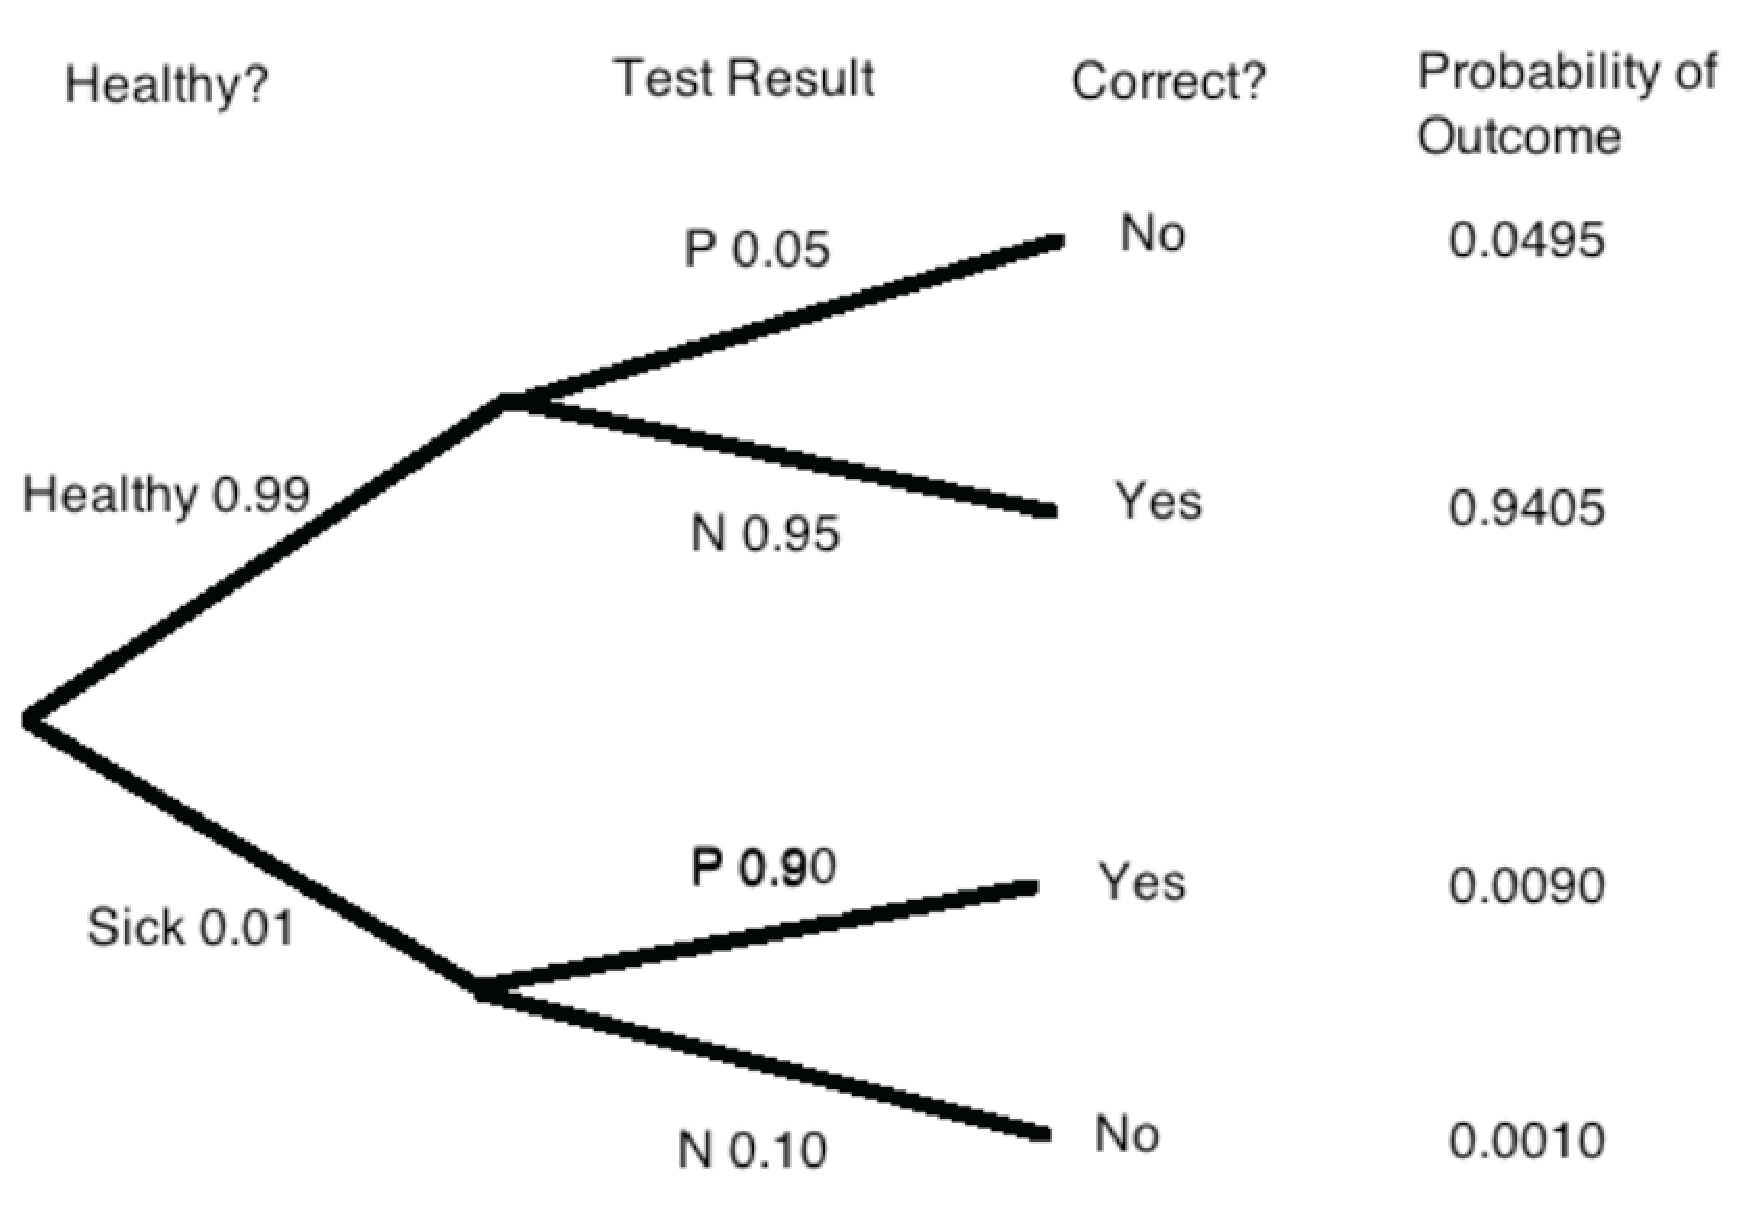
\includegraphics[width=.9\textwidth]{figures/drafts/mammo-tree}}
\caption{The tree diagram for a breast cancer test.}
\label{fig:15C1}
\end{figure}

\iffalse  %premature, total probability in next section.
Notice that the test gives the correct answer with probability $0.9405
+ 0.009 = 0.9495$.
\fi

\paragraph{Step 2: Define Events of Interest}

Let $A$ be the event that the person has breast cancer.  Let $B$ be the
event that the test was positive.  The outcomes in each event are marked
in the tree diagram.  We want to find $\prcond{A}{B}$, the probability
that a person has breast cancer, given that the test was positive.

\paragraph{Step 3: Find Outcome Probabilities}

First, we assign probabilities to edges.  These probabilities are
drawn directly from the problem statement.  By the Product Rule, the
probability of an outcome is the product of the probabilities on the
corresponding root-to-leaf path.  All probabilities are shown in
Figure~\ref{fig:15C1}.

\paragraph{Step 4: Compute Event Probabilities}

From Definition~\ref{LN12:prcond}, we have
\begin{equation*}
\prcond{A}{B}	= \frac{\pr{A \intersect B}}{\pr{B}} %\\[2pt]
		= \frac{0.009}{0.009 + 0.0495} %\\[2pt]
		\approx 15.4\%.
\end{equation*}
So, if the test is positive, then there is an 84.6\% chance that the
result is incorrect, even though the test is nearly 95\% accurate!  So
this seemingly pretty accurate test doesn't tell us much.  To see why
percent accuracy is no guarantee of value, notice that there is a
simple way to make a test that is 99\% accurate: always return a
negative result!  This test gives the right answer for all healthy
people and the wrong answer only for the 1\% that actually have
cancer.  This 99\% accurate test tells us nothing; the ``less
accurate'' mammogram is still a lot more useful.


\begin{editingnotes}
There is a similar ``paradox'' in weather forecasting.  During winter,
almost all days in Boston are wet and overcast.  Predicting miserable
weather every day may be more accurate than really trying to get it
right!
\end{editingnotes}


\begin{editingnotes}
\textbf{Eli:} This needs a ``this just goes to show'' lesson here, but
I'm not actually sure what that lesson should be.
\end{editingnotes}

\subsection{Natural Frequencies}

That there is only about a 15\% chance that the patient actually has
the condition when the test say so may seem surprising at first, but
it makes sense with a little thought.  There are two ways the patient
could test positive: first, the patient could have the condition and
the test could be correct; second, the patient could be healthy
and the test incorrect.  But almost everyone is healthy!  The number
of healthy individuals is so large that even the mere 5\% with false
positive results overwhelm the number of genuinely positive results
from the truly ill.

Thinking like this in terms of these ``natural frequencies'' can be a
useful tool for interpreting some of the strange seeming results
coming from those formulas.  For example, let's take a closer look at
the mammogram example.

Imagine 10,000 women in our demographic.  Based on the frequency of
the disease, we'd expect 100 of them to have breast cancer.  Of those,
90 would have a positve result.  The remaining 9,900 woman are
healthy, but 5\% of them---500, give or take---will show a false
positive on the mammogram.  That gives us 90 real positives out of a
little fewer than 600 positives.  An 85\% error rate isn't so
surprising after all.

\begin{editingnotes}
Add a box or problem with an example where this test would be useful.
For example, if you have only enough medicine to treat half the
population, and you randomly choose people to treat, then the
probability that you treat a sick person will be 1/2.  But if you
first treat all the people who test positive, the probability that a
sick person will be treated will be nearly 0.9.
\end{editingnotes}


\subsection{\emph{A Posteriori} Probabilities}\label{aposteriori_subsec}

If you think about it much, the medical testing problem we just
considered could start to trouble you.  You may wonder if a statement
like ``If someone tested positive, then that person has the condition
with probability~18\%'' makes sense, since a given person being tested
either has the disease or they don't.

\begin{editingnotes}
ARM: THIS IS A LITTLE SLOPPY; REVISE:
\end{editingnotes}

One way to understand such a statement is that it just means that 15\%
of the people who test positive will actually have the condition.  Any
particular person has it or they don't, but a \emph{randomly selected}
person among those who test positive will have the condition with
probability~15\%.

But what does this~15\% probability tell you if you \emph{personally}
got a positive result?  Should you be relieved that there is less than
one chance in five that you have the disease?  Should you worry that
there is nearly one chance in five that you do have the disease?
Should you start treatment just in case?  Should you get more tests?

These are crucial practical questions, but it is important to
understand that they are not \emph{mathematical} questions.  Rather,
these are questions about statistical judgements and the philosophical
meaning of probability.  We'll say a bit more about this after looking
at one more example of after-the-fact probabilities.

\begin{editingnotes}
Cite a source that discusses the philosophy of statistics.
\end{editingnotes}

\iffalse
Anyway, if the after-the-fact nature of the medical testing example
bothers you, you will definitely be worried by the following,
which goes even further down this path.
\fi

\subsubsection{The Hockey Team in Reverse}\label{reverse-hockey}

Suppose that we turn the hockey question around: what is the
probability that the local C-league hockey team won their first game,
given that they won the series?

As we discussed earlier, some people find this question absurd.  If
the team has already won the tournament, then the first game is long
since over.  Who won the first game is a question of fact, not of
probability.  However, our mathematical theory of probability contains
no notion of one event preceding another.  There is no notion of time
at all.  Therefore, from a mathematical perspective, this is a
perfectly valid question.  And this is also a meaningful question from
a practical perspective.  Suppose that you're told that the local team
won the series, but not told the results of individual games.  Then,
from your perspective, it makes perfect sense to wonder how likely it
is that local team won the first game.

A conditional probability $\prcond{B}{A}$ is called  \term{a
posteriori} if event $B$ precedes event $A$ in time.  Here are some
other examples of a posteriori probabilities:
%
\begin{itemize}
\item The probability it was cloudy this morning, given that it rained
in the afternoon.
\item The probability that I was initially dealt two queens in Texas
No Limit Hold 'Em poker, given that I eventually got four-of-a-kind.
\end{itemize}
% Mathematically, a posteriori probabilities are \emph{no different}
from ordinary probabilities; the distinction comes from our view of
causality, which is a philosophical question rather than a
mathematical one.

\iffalse Our only reason for drawing attention to them is to say,
``Don't let them rattle you.''\fi

Let's return to the original problem.  The probability that the
local team won their first game, given that they won the series
is $\prcond{B}{A}$.  We can compute this using the definition of
conditional probability and the tree diagram in Figure~\ref{fig:15B2}:
%
\begin{align*}
\prcond{B}{A}  = \frac{\pr{B \intersect A}}{\pr{A}} %\\[2pt]
               = \frac{1/3 + 1/18}{1/3 + 1/18 + 1/9} %\\[2pt]
               = \frac{7}{9}.
\end{align*}

\begin{editingnotes}
\TBA{MOVE TO A PROBLEM}

This answer is suspicious.  In the preceding section, we showed that
$\prcond{A}{B}$ was also $7/9$.  Some reflection suggests that
$\prcond{A}{B} = \prcond{B}{A}$ is unlikely to be true in general.
For example, the probability that I feel uneasy, given that I was
abducted by aliens, is pretty large.  But the probability that I was
abducted by aliens, given that I feel uneasy, is rather small.

Let's work out the general conditions under which $\prcond{A}{B} =
\prcond{B}{A}$.  By the definition of conditional probability, this
equation holds if an only if:
%
\[
\frac{\pr{A \intersect B}}{\pr{B}} = \frac{\pr{A \intersect B}}{\pr{A}}
\]
%
This equation, in turn, holds only if the denominators are equal or
the numerator is~0; namely if
%
\[
\pr{B} = \pr{A}
\hspace{0.25in} \text{or} \hspace{0.25in}
\pr{A \intersect B} = 0.
\]
%
The former condition holds in the hockey example; the probability that
the local team wins the series (event~$A$) is equal to the
probability that it wins the first game (event~$B$) since both
probabilities are~$1/2$.
\end{editingnotes}

In general, such pairs of probabilities are related by \idx{Bayes'
  Rule}:
%
\begin{theorem}[Bayes' Rule]
%If $\pr{A}$ and $\pr{B}$ are nonzero, then:
%
\begin{equation}\label{bayesrule}
    \prcond{B}{A} = \frac{\prcond{A}{B} \cdot \pr{B}}{\pr{A}}
\end{equation}
\end{theorem}

\begin{proof}
%When $\pr{A}$ and $\pr{B}$ are nonzero,
We have
\[
\prcond{B}{A} \cdot \pr{A} = \prob{A \intersect B} = \prcond{A}{B} \cdot \pr{B}
\]
by definition of conditional probability.  Dividing by $\prob{A}$
gives~\eqref{bayesrule}.
\end{proof}

\subsection{Philosphy of Probability}

Let's try to assign a probability to the event
%
\[
[2^{6972607} - 1 \text{ is a prime number}]
\]
It's not obvious how to check whether such a large number is prime, so
you might try an estimation based on the density of primes.  The Prime
Number Theorem implies that only about $1$ in 5 million numbers in
this range are prime, so you might say that the probability is about
$2 \cdot 10^{-8}$.  On the other hand, given that we chose this
example to make some philosophical point, you might guess that we
probably purposely chose an obscure looking prime number, and you
might be willing to make an even money bet that the number is prime.
In other words, you might think the probability is 1/2.  Finally, we
can take the position that assigning a probability to this statement
is nonsense because there is no randomness involved; the number is
either prime or it isn't.  This is the view we take in this text.

An alternate view is the \term{Bayesian} approach, in which a
probability is interpreted as a \emph{degree of belief} in a
proposition.  A Bayesian would agree that the number above is either
prime or composite, but they would be perfectly willing to assign a
probability to each possibility.  The Bayesian approach is very broad
in its willingness to assign probabilities to any event, but the
problem is that there is no single ``right'' probability for an event,
since the probability depends on one's initial beliefs.  On the other
hand, if you have confidence in some set of initial beliefs, then
Bayesianism provides a convincing framework for updating your beliefs
as further information emerges.

As an aside, it is not clear whether Bayes himself was Bayesian in
this sense.  However, a Bayesian would be willing to talk about the
probability that Bayes was Bayesian.

Another school of thought says that probabilities can only be
meaningfully applied to \emph{repeatable processes} like rolling dice
or flipping coins.  In this \term{frequentist} view, the probability
of an event represents the fraction of trials in which the event
occurred.  So we can make sense of the \emph{a posteriori}
probabilities of the C-league hockey example of
Section~\ref{reverse-hockey} by imagining that many hockey series were
played, and the probability that the local team won their first game,
given that they won the series, is simply the fraction of series where
they won the first game among all the series they won.

Getting back to prime numbers, we mentioned in
Section~\ref{probable_primes} that there is a probabilistic primality
test.  If a number $N$ is composite, there is at least a $3/4$ chance
that the test will discover this.  In the remaining $1/4$ of the time,
the test is inconclusive.  But as long as the result is inconclusive,
the test can be run independently again and again up to, say, 100
times.  So if $N$ actually is composite, then the probability that
$000$ repetitions of the probabilistic test do not discover this is
at most:
\[
\paren{\frac{1}{4}}^{100}.
\]
If the test remained inconclusive after 100 repetitions, it is still
logically possible that $N$ is composite, but betting that $N$ is
prime would be the best bet you'll ever get to make!  If you're
comfortable using probability to describe your personal belief about
primality after such an experiment, you are being a Bayesian.  A
frequentist would not assign a probability to $N$'s primality, but
they would also be happy to bet on primality with tremendous
confidence.  We'll examine this issue again when we discuss polling
and confidence levels in Section~\ref{sec: Confidence_v_Prob}.

Despite the philosophical divide, the real world conclusions Bayesians
and Frequentists reach from probabilities are pretty much the same,
and even where their interpretations differ, they use the same theory
of probability.

\iffalse

Next, let's look at a problem that even bothers us.

\subsection{A Coin Problem}

Suppose that someone hands you either a fair coin or a trick coin with
heads on both sides.  You flip the coin 100 times and see heads every
time.  What can you say about the probability that you flipped the
fair coin?  Remarkably, nothing!

In order to make sense out of this outrageous claim, let's formalize
the problem.  The sample space is worked out in the tree diagram shown
in Figure~\ref{fig:15C2}.  We do not know the probability~$p$ that you
were handed the fair coin initially---you were just given one coin or
the other.
%
\begin{figure}[h]

\graphic{trick-coin}

\caption{The tree diagram for the coin-flipping problem.}

\label{fig:15C2}

\end{figure}
%
Let $A$ be the event that you were handed the fair coin, and let $B$
be the event that you flipped 100 straight heads.  We're looking
for $\prcond{A}{B}$, the probability that you were handed the fair
coin, given that you flipped 100 heads.  The outcome probabilities are
worked out in Figure~\ref{fig:15C2}.  Plugging the results into the
definition of conditional probability gives:
%
\begin{align*}
\prcond{A}{B}	& = \frac{\pr{A \intersect B}}{\pr{B}} \\[2pt]
		& = \frac{p / 2^{100}}{1 - p + p / 2^{100}} \\[2pt]
		& = \frac{p}{2^{100} (1 - p) + p}.
\end{align*}
%
This expression is very small for moderate values of $p$ because of
the $2^{100}$ term in the denominator.  For example, if $p = 1/2$,
then the probability that you were given the fair coin is essentially
zero.

But we \emph{do not know} the probability $p$ that you were given
the fair coin.  And perhaps the value of $p$ is \emph{not} moderate;
in fact, maybe $p = 1 - 2^{-100}$.  Then there is nearly an even
chance that you have the fair coin, given that you flipped 100 heads.
In fact, maybe you were handed the fair coin with probability $p = 1$.
Then the probability that you were given the fair coin is, well, one!

Of course, it is extremely unlikely that you would flip 100 straight
heads, but in this case, that is a given from the assumption of the
conditional probability.  And so if you really did see 100 straight
heads, it would be very tempting to also assume that $p$~is not close
to~1 and hence that you are very likely to have flipped the trick
coin.

We will encounter a very similar issue when we look at methods for
estimation by sampling in Section~\ref{sec:sampling}.
\fi

%\subsection{Conditional Identities}

\begin{problems}
\homeworkproblems
\pinput{PS_conditional_probability_product_rule}
\end{problems}

\section{The Law of Total Probability}\label{sec:total_probability}

Breaking a probability calculation into cases simplifies many
problems.  The idea is to calculate the probability of an event $A$ by
splitting into two cases based on whether or not another event $E$
occurs.  That is, calculate the probability of $A\nobreak
\intersect\nobreak E$ and $A \intersect \setcomp{E}$.  By the Sum
Rule, the sum of these probabilities equals $\pr{A}$.  Expressing the
intersection probabilities as conditional probabilities yields:
\begin{rul}[Law of Total Probability: single event]\label{total_prob_Ebar}
%If $\prob{E}$ and $\prob{\setcomp{E}}$~are nonzero, then
\[
\pr{A} = \prcond{A}{E} \cdot \pr{E} +
         \prcond{A}{\setcomp{E}} \cdot \pr{\setcomp{E}}.
\]
\end{rul}

For example, suppose we conduct the following experiment.  First, we
flip a fair coin.  If heads comes up, then we roll one die and take the
result.  If tails comes up, then we roll two dice and take the sum of
the two results.  What is the probability that this process yields a
2?  Let $E$ be the event that the coin comes up heads, and let $A$ be
the event that we get a 2 overall.  Assuming that the coin is fair,
$\pr{E} = \pr{\setcomp{E}} = 1/2$.  There are now two cases. If we
flip heads, then we roll a 2 on a single die with probability
$\prcond{A}{E} = 1/6$.  On the other hand, if we flip tails, then we
get a sum of 2 on two dice with probability
$\prcond{A}{\setcomp{E}} = 1/36$.  Therefore, the probability that
the whole process yields a 2 is
\[
\pr{A} = \frac{1}{2} \cdot \frac{1}{6} + \frac{1}{2} \cdot \frac{1}{36} =
  \frac{7}{72}.
\]

This rule extends to any set of disjoint events that make up the
entire sample space.  For example,
\begin{rul*}[Law of Total Probability: 3-events]
If $E_1, E_2,$ and $E_3$ are disjoint and
$\pr{E_1 \union E_2 \union E_3} = 1$, then
\[
\pr{A} = \prcond{A}{E_1} \cdot \pr{E_1} + \prcond{A}{E_2} \cdot
\pr{E_2} + \prcond{A}{E_3} \cdot \pr{E_3}\,.
\]
\end{rul*}
This in turn leads to a three-event version of Bayes' Rule in which
the probability of event $E_1$ given $A$ is calculated from the
``inverse'' conditional probabilities of $A$ given $E_1$, $E_2$, and
$E_3$:

\begin{rul*}[Bayes' Rule: 3-events]
\[
\prcond{E_1}{A} = \frac{\prcond{A}{E_1}\cdot \pr{E_1}}
                       {\prcond{A}{E_1} \cdot \pr{E_1} +
                        \prcond{A}{E_2} \cdot \pr{E_2} +
                        \prcond{A}{E_3} \cdot \pr{E_3}}
\]
\end{rul*}

The generalization of these rules to $n$ disjoint events is a routine
exercise (Problems~\ref{TP_multi_total_prob} and~\ref{TP_bayes_proof}).

\subsection{Conditioning on a Single Event}\label{cond_ident_subsec}

The probability rules that we derived in Section~\ref{sec:union_bound}
extend to probabilities conditioned on the same event.  For example,
the Inclusion-Exclusion formula for two sets holds when all
probabilities are conditioned on an event $C$:
\[
\prcond{A \union B}{C} = \prcond{A}{C} + \prcond{B}{C} - \prcond{A \intersect B}{C}.
\]
This is easy to verify by plugging in the Definition~\ref{LN12:prcond}
of conditional 
probability.\footnote{Problem~\ref{PS_conditional_space} explains why
  this and similar conditional identities follow on general principles
  from the corresponding unconditional identities.}

\iffalse
%This follows from the fact that if $\pr{C} \neq 0$, then
Namely,
\begin{align*}
\prcond{A \union B}{C}
    &= \frac{\pr{(A \union B) \intersect C}}{\pr{C}} \\[3pt]
    &= \frac{\pr{(A \intersect C) \union (B \intersect C)}}{\pr{C}} \\[3pt]
    &= \frac{\pr{A \intersect C} + \pr{B \intersect C}
             - \pr{A \intersect B \intersect C}}
            {\pr{C}} \\[3pt]
    &= \prcond{A}{C} + \prcond{B}{C} - \prcond{A \intersect B}{C}.
\end{align*}
\fi

It is important not to mix up events before and after the conditioning
bar.  For example, the following is \emph{not} a valid identity:
%
\begin{falseclm*}
\begin{equation}\label{LN12:fc}
\prcond{A}{B \union C} = \prcond{A}{B} + \prcond{A}{C} - \prcond{A}{B \intersect C}.
\end{equation}
\end{falseclm*}

A simple counter-example is to let $B$ and $C$ be events over a
uniform space with most of their outcomes in $A$, but not overlapping.
This ensures that $\prcond{A}{B}$ and $\prcond{A}{C}$ are both close
to 1.  For example,
\begin{align*}
B & \eqdef \Zintv{0}{9},\\
C & \eqdef \Zintv{10}{18} \union \set{0},\\
A & \eqdef \Zintv{1}{18},
\end{align*}
so
\[
\prcond{A}{B} = \frac{9}{10} = \prcond{A}{C}.
\]
Also, since 0 is the only outcome in $B \intersect C$ and $0 \notin
A$, we have
\[
\prcond{A}{B \intersect C} = 0
\]
So the right-hand side of~\eqref{LN12:fc} is 1.8, while the left-hand
side is a probability which can be at most 1---actually, it is 18/19.

\iffalse

A counterexample is shown in Figure~\ref{fig:15D2}.  In this case,
$\prcond{A}{B} = 1/2$, $\prcond{A}{C} = 1/2$, $\prcond{A}{B \intersect
  C} = 1$, and $\prcond{A}{B \union C} = 1/3$.  However, since
$1/3 \ne 1/2 + 1/2 - 1$, equation~\eqref{LN12:fc} does not hold.
%
\begin{figure}

\graphic{cx19}

\caption{A counterexample to equation~\eqref{LN12:fc}.  Event~$A$ is
  the dark-bordered rectangle, event~$B$ is the rectangle with
  vertical stripes, and event~$C$ is the rectangle with horizontal
  stripes.  $B \intersect C$ lies entirely within~$A$ while $B - C$
  and $C - B$ are entirely outside of~$A$.}

\label{fig:15D2}

\end{figure}
\fi

\begin{problems}
\practiceproblems
\pinput{TP_six_shooter_probability}
\pinput{TP_multi_total_prob}
\pinput{TP_bayes_proof}

\classproblems
\pinput{CP_missing_card_probability}
\pinput{PS_conditional_aces}
\pinput{CP_conditional_prob_says_so_bug}
\pinput{FP_skywalker_prob_lin_recur_gen_func}
\pinput{FP_directed_graphs_and_probability}

\homeworkproblems
\pinput{PS_levitating_LAs}
\pinput{PS_conditional_probability_problem_errors}
\pinput{CP_coin_flip_sequences}
\pinput{PS_13_card_hand}
\pinput{PS_conditional_space}
\pinput{PS_red_black_card_strategy}

\examproblems
\pinput{FP_college_probability}
\pinput{FP_monty_hall_variant}
\pinput{FP_conditional_prob_inequality}
\pinput{MQ_conditional_prob_inequality}
\pinput{FP_conditional_beaver_fever}
\pinput{FP_red_and_blue_goats}
\pinput{FP_neighborhood_census}
\pinput{MQ_voldemort_returns}
\pinput{FP_random_grid_walk}
\end{problems}

\section{Simpson's Paradox}\label{discrimination_subsec}

In 1973, a famous university was investigated for gender
discrimination~\cite{Berkeley75}.  The investigation was prompted by
evidence that, at first glance, appeared definitive: in 1973, 44\% of
male applicants to the school's graduate programs were accepted, but
only 35\% of female applicants were admitted.

However, this data turned out to be completely misleading.  Analysis
of the individual departments, showed not only that few showed
significant evidence of bias, but also that among the few departments
that \emph{did} show statistical irregularities, most were slanted
\emph{in favor of women}.  This suggests that if there was any sex
discrimination, then it was against men!

Given the discrepancy in these findings, it feels like someone must be
doing bad math---intentionally or otherwise.  But the numbers are not
actually inconsistent.  In fact, this statistical hiccup is common
enough to merit its own name: \term{Simpson's Paradox} occurs when
multiple small groups of data all exhibit a similar trend, but that
trend reverses when those groups are aggregated.  To explain how this
is possible, let's first clarify the problem by expressing both
arguments in terms of conditional probabilities.  For simplicity,
suppose that there are only two departments EE and CS.  Consider the
experiment where we pick a random candidate.  Define the following
events:
%
\begin{itemize}
\item $A \eqdef$ the candidate is admitted to his or her program of choice,
\item $F_{EE} \eqdef$ the candidate is a woman applying to the EE department,
\item $F_{CS} \eqdef$ the candidate is a woman applying to the CS department,
\item $M_{EE} \eqdef$ the candidate is a man applying to the EE department,
\item $M_{CS} \eqdef$ the candidate is a man applying to the CS department.
\end{itemize}
Assume that all candidates are either men or women, and that no
candidate belongs to both departments. That is,  the events $F_{EE}$,
$F_{CS}$, $M_{EE}$, and $M_{CS}$ are all disjoint.

In these terms, the plaintiff's assertion---that a male candidate is
more likely to be admitted to the university than a female---can be
expressed by the following inequality:
\[
    \prcond{A}{M_{EE} \union M_{CS}} > \prcond{A}{F_{EE} \union F_{CS}}.
\]

The university's retort that \emph{in any given department}, a male
applicant is less likely to be admitted than a female can be expressed
by a pair of inequalities:
\begin{align*}
\prcond{A}{M_{EE}} & < \prcond{A}{F_{EE}} \quad\text{and}\\
\prcond{A}{M_{CS}} & < \prcond{A}{F_{CS}}.
\end{align*}

We can explain how there could be such a discrepancy between
university-wide and department-by-department admission statistics by
supposing that the CS department is more selective than the EE
department, but CS attracts a far larger number of woman applicants
than EE.\footnote{At the actual university in the lawsuit, the
  ``exclusive'' departments more popular among women were those that
  did not require a mathematical foundation, such as English and
  education.  Women's disproportionate choice of these careers
  reflects gender bias, but one which predates the university's
  involvement.}.  Table~\ref{fig:15D3} shows some admission statistics
for which the inequalities asserted by both the plaintiff and the
university hold.

\begin{table}

\begin{tabular}{crr}
CS & 2 men admitted out of 5 candidates      &   40\% \\
   & 50 women admitted out of 100 candidates     &  50\% \\
EE & 70 men admitted out of 100 candidates   &  70\% \\
   & 4 women admitted out of 5 candidates         & 80\% \\
\hline
Overall & 72 men admitted, 105 candidates & $\approx 69\%$ \\
        & 54 women admitted, 105 candidates   & $\approx 51\%$
\end{tabular}

\caption{A scenario in which men are overall more likely than women to
  be admitted to a school, despite being less likely to be admitted
  into any given program.}

\label{fig:15D3}

\end{table}

Initially, we and the plaintiffs both assumed that the overall
admissions statistics for the university could only be explained by
gender discrimination.  The department by department statistics seems
to belie the accusation of discrimination.  But do they really?

Suppose we replaced ``the candidate is a man/woman applying to the EE
department,'' by ``the candidate is a man/woman for whom an admissions
decision was made during an odd-numbered day of the month,'' and
likewise with CS and an even-numbered day of the month.  Since we
don't think the parity of a date is a cause for the outcome of an
admission decision, we would most likely dismiss the ``coincidence''
that on both odd and even dates, women are more frequently admitted.
Instead we would judge, based on the overall data showing women less
likely to be admitted, that gender bias against women \emph{was} an
issue in the university.

Bear in mind that it would be the \emph{same numerical data} that we
would be using to justify our different conclusions in the
department-by-department case and the even-day-odd-day case.  We
interpreted the same numbers differently based on our implicit causal
beliefs, specifically that departments matter and date parity does
not.  It is circular to claim that the data corroborated our beliefs
that there is or is not discrimination.  Rather, our interpretation of
the data correlation depended on our beliefs about the causes of
admission in the first place.\footnote{These issues are thoughtfully
  examined in \emph{Causality: Models, Reasoning and Inference}, Judea
  Pearl, Cambridge U. Press, 2001.}  This example highlights a basic
principle in statistics which people constantly ignore: \emph{never
  assume that correlation implies causation}.
\begin{problems}
\practiceproblems
\pinput{TP_bogus_discrimination_contradiction}
\end{problems}

\section{Independence}\label{sec:independence}
Suppose that we flip two fair coins simultaneously on opposite sides
of a room.  Intuitively, the way one coin lands does not affect the
way the other coin lands.  The mathematical concept that captures
this intuition is called \term{independence}.
\begin{definition}\label{def:independence}
An event with probability 0 is defined to be independent of every
event (including itself).  If $\pr{B} \neq 0$, then
event $A$ is independent of event $B$ iff
\begin{equation}\label{eqn:independence}
    \prcond{A}{B} = \pr{A}.
\end{equation}
\end{definition}
In other words, $A$ and~$B$ are independent if knowing that $B$
happens does not alter the probability that $A$~happens, as is the
case with flipping two coins on opposite sides of a room.

\subsubsection*{Potential Pitfall}

Students sometimes get the idea that disjoint events are independent.
The \emph{opposite} is true: if $A \intersect B = \emptyset$, then
knowing that $A$ happens means you know that $B$ does not happen.
Disjoint events are \emph{never} independent---unless one of them has
probability zero.

\subsection{Alternative Formulation}

Sometimes it is useful to express independence in an alternate form
which follows immediately from Definition~\ref{def:independence}:

\begin{theorem}\label{thm:16A1}
$A$ is independent of~$B$ if and only if
\begin{equation}\label{eqn:15D3}
    \pr{A \intersect B} = \pr{A} \cdot \pr{B}.
\end{equation}
\end{theorem}

Notice that Theorem~\ref{thm:16A1} makes apparent the symmetry between
$A$ being independent of $B$ and $B$ being independent of $A$:
\begin{corollary}
$A$ is independent of $B$ iff $B$ is independent of $A$.
\end{corollary}


\iffalse

\begin{proof}
There are two cases to consider depending on whether or not $\prob{B} =
0$.
\begin{description}

\item[Case 1 $(\prob{B} = 0)$:]
If $\prob{B} = 0$, $A$ and~$B$ are independent by
Definition~\ref{def:independence}.  In addition,
equation~\eqref{eqn:15D3} holds since both sides are~0.  Hence, the
theorem is true in this case.

\item[Case 2 $(\prob{B} > 0)$:]
By Definition~\ref{LN12:prcond},
\begin{equation*}
    \prob{A \cap B} = \prcond{A}{B} \prob{B}.
\end{equation*}
So equation~\eqref{eqn:15D3} holds if
\begin{equation*}
    \prcond{A}{B} = \prob{A},
\end{equation*}
which, by Definition~\ref{def:independence}, is true iff $A$ and~$B$
are independent.  Hence, the theorem is true in this case as well.
\qedhere
\end{description}
\end{proof}
\fi

\subsection{Independence Is an Assumption}

Generally, independence is something that you \emph{assume} in
modeling a phenomenon.  For example, consider the experiment of
flipping two fair coins.  Let $A$~be the event that the first coin
comes up heads, and let $B$~be the event that the second coin is
heads.  If we assume that $A$ and~$B$ are independent, then the
probability that both coins come up heads is:
%
\begin{equation*}
\pr{A \intersect B}  = \pr{A} \cdot \pr{B} %\\[2pt]
               = \frac{1}{2} \cdot \frac{1}{2} %\\[2pt]
               = \frac{1}{4}.
\end{equation*}

In this example, the assumption of independence is reasonable.  The
result of one coin toss should have negligible impact on the outcome
of the other coin toss.  And if we were to repeat the experiment many
times, we would be likely to have~$A \cap B$ about~1/4 of the time.

On the other hand, there are many examples of events where assuming
independence isn't justified.  For example, an hourly weather forecast
for a clear day might list a 10\% chance of rain every hour from noon
to midnight, meaning each hour has a 90\% chance of being dry.  But
that does \emph{not} imply that the odds of a rainless day are a mere
$0.9^{12} \approx 0.28$.  In reality, if it doesn't rain as of 5pm,
the odds are higher than 90\% that it will stay dry at 6pm as
well---and if it starts pouring at 5pm, the chances are much higher
than 10\% that it will still be rainy an hour later.


\iffalse
let $C$~be the
event that tomorrow is cloudy and $R$ be the event that tomorrow is
rainy.  Perhaps $\pr{C} = 1/5$ and $\pr{R} = 1/10$ in Boston.  If
these events were independent, then we could conclude that the
probability of a rainy, cloudy day was quite small:
%
\begin{equation*}
\pr{R \intersect C} = \pr{R} \cdot \pr{C} % \\[2pt]
               = \frac{1}{5} \cdot \frac{1}{10} % \\[2pt]
               = \frac{1}{50}.
\end{equation*}
%
Unfortunately, these events are definitely not independent; in
particular, every rainy day is cloudy.  Thus, the probability of a
rainy, cloudy day is actually~$1/10$.
\fi

Deciding when to \emph{assume} that events are independent is a tricky
business.  In practice, there are strong motivations to assume
independence since many useful formulas (such as
equation~\eqref{eqn:15D3}) only hold if the events are independent.
But you need to be careful:
\iffalse
 lest you end up deriving false conclusions.
\fi
we'll describe several famous examples where (false) assumptions of
independence led to trouble.
\iffalse
 over the next several chapters
\fi
This problem gets even trickier when there are more than two events in
play.

\begin{problems}
\practiceproblems
\pinput{TP_independence_size}
\pinput{TP_conditional_independence}

\classproblems
\pinput{CP_independent_evidence}
\pinput{CP_graph_logic_probability_S16}

\end{problems}

\section{Mutual Independence}\label{sec:mutual}

%\subsection{Definition}

We have defined what it means for two events to be independent.  What
if there are more than two events?  For example, how can we say that
the flips of $n$~coins are all independent of one another?  A set of
events is said to be \term{mutually independent} if the probability of
each event in the set is the same no matter which of the other events
has occurred.  This is equivalent to saying that for any selection of
two or more of the events, the probability that all the selected
events occur equals the product of the probabilities of the selected
events.

For example, four events~$E_1, E_2, E_3, E_4$ are mutually
independent if and only if all of the following equations hold:
%
\begin{align*}
\pr{E_1 \intersect E_2}
    & = \pr{E_1} \cdot \pr{E_2}
\\
\pr{E_1 \intersect E_3}
    & = \pr{E_1} \cdot \pr{E_3}
\\
\pr{E_1 \intersect E_4}
    & = \pr{E_1} \cdot \pr{E_4}
\\
\pr{E_2 \intersect E_3}
    & = \pr{E_2} \cdot \pr{E_3}
\\
\pr{E_2 \intersect E_4}
    & = \pr{E_2} \cdot \pr{E_4}
\\
\pr{E_3 \intersect E_4}
    & = \pr{E_3} \cdot \pr{E_4}
 \\
\pr{E_1 \intersect E_2 \intersect E_3}
    & = \pr{E_1} \cdot \pr{E_2} \cdot \pr{E_3}
\\
\pr{E_1 \intersect E_2 \intersect E_4}
    & = \pr{E_1} \cdot \pr{E_2} \cdot \pr{E_4}
\\
\pr{E_1 \intersect E_3 \intersect E_4}
    & = \pr{E_1} \cdot \pr{E_3} \cdot \pr{E_4}
\\
\pr{E_2 \intersect E_3 \intersect E_4}
    & = \pr{E_2} \cdot \pr{E_3} \cdot \pr{E_4}
 \\
\pr{E_1 \intersect E_2 \intersect E_3 \intersect E_4} & = \pr{E_1} \cdot \pr{E_2} \cdot \pr{E_3} \cdot \pr{E_4}
\end{align*}

The generalization to mutual independence of $n$ events should now be clear.

\begin{editingnotes}
MAKE INTO A PROBLEM:

We could formalize this with conditional probabilities
as in Definition~\ref{def:independence}, but we'll jump directly to
the cleaner definition based on products of probabilities as in
Theorem~\ref{thm:16A1}:

\begin{definition}\label{def:mutual_independence}
A set of events~$E_1, E_2, \dots, E_n$, is \term{mutually independent}
if $\forall i \in \Zintv{1}{n}$ and $\forall S \subseteq \Zintv{1}{n} - \set{i}$,
either
\begin{equation*}
    \Prob{\bigcap_{j \in S} E_j} = 0
\quad
\text{or}
\quad
    \prob{E_i} = \prcond{E_i}{\bigcap_{j \in S} E_j}.
\end{equation*}
\end{definition}

\subsection{Alternative Formulation}

Just as Theorem~\ref{thm:16A1} provided an alternative definition of
independence for two events, there is an alternative definition for
mutual independence.

%\begin{theorem}\label{thm:16A2}

\begin{definition}\label{def:mutual_indep}
A set of events~$E_1, E_2, \dots, E_n$ is mutually independent iff
for all subsets $S \subseteq \Zintv{1}{n}$,
\begin{equation*}
    \Prob{\bigcap_{j \in S} E_j} = \prod_{j \in S} \prob{E_j}.
\end{equation*}
\end{definition}

%\end{theorem}
\iffalse
The proof of Theorem~\ref{thm:16A2} uses induction and reasoning
similar to the proof of Theorem~\ref{thm:16A1}.  We will not include
the details here.
\fi

Definition~\ref{def:mutual_indep} says that $E_1, E_2, \dots, E_n$~are
mutually independent if and only if all of the following equations
hold for all distinct $i$, $j$, $k$ and~$l$:
%
\begin{align*}
\pr{E_i \intersect E_j}
    & = \pr{E_i} \cdot \pr{E_j}
%    & \text{for all distinct $i$, $j$}
 \\
\pr{E_i \intersect E_j \intersect E_k}
    & = \pr{E_i} \cdot \pr{E_j} \cdot \pr{E_k}
%     & \text{for all distinct $i$, $j$, $k$}
 \\
\pr{E_i \intersect E_j \intersect E_k \intersect E_l}
    & = \pr{E_i} \cdot \pr{E_j} \cdot \pr{E_k} \cdot \pr{E_l}
%    & \text{for all distinct $i$, $j$, $k$, $l$}
 \\
    & \XasWideAsY{\vdots}{${}={}$} \\
\pr{E_1 \intersect \cdots \intersect E_n} & = \pr{E_1} \cdots \pr{E_n}.
\end{align*}

For example, if we toss $n$~fair coins, the tosses are mutually
independent iff for every subset of~$m$~coins, the probability that
every coin in the subset comes up heads is~$2^{-m}$.
\end{editingnotes}

\subsection{DNA Testing}

Assumptions about independence are routinely made in practice.
Frequently, such assumptions are quite reasonable.  Sometimes,
however, the reasonableness of an independence assumption is not so
clear, and the consequences of a faulty assumption can be severe.

Let's return to the O. J. Simpson murder trial.  The following expert
testimony was given on May 15, 1995:
\begin{description}

\item[Mr. Clarke:] When you make these estimations of frequency---and
I believe you touched a little bit on a concept called independence?

\item[Dr. Cotton:] Yes, I did.

\item[Mr. Clarke:] And what is that again?

\item[Dr. Cotton:] It means whether or not you inherit one allele that
  you have is not---does not affect the second allele that you might
  get.  That is, if you inherit a band at 5,000 base pairs, that
  doesn't mean you'll automatically or with some probability inherit
  one at 6,000.  What you inherit from one parent is [independent of]
  what you inherit from the other.

\item[Mr. Clarke:] Why is that important?

\item[Dr. Cotton:] Mathematically that's important because if that
were not the case, it would be improper to multiply the frequencies
between the different genetic locations.

\item[Mr. Clarke:] How do you---well, first of all, are these markers
independent that you've described in your testing in this case?

\end{description}

Presumably, this dialogue was as confusing to you as it was for the
jury.  Essentially, the jury was told that genetic markers in blood
found at the crime scene matched Simpson's.  Furthermore, they were
told that the probability that the markers would be found in a
randomly-selected person was at most 1 in 170 million.  This
astronomical figure was derived from statistics such as:
%
\begin{itemize}
\item 1 person in 100 has marker $A$.
\item 1 person in 50 marker $B$.
\item 1 person in 40 has marker $C$.
\item 1 person in 5 has marker $D$.
\item 1 person in 170 has marker $E$.
\end{itemize}
%
Then these numbers were multiplied to give the probability that a
randomly-selected person would have all five markers:
\begin{align*}
\pr{A \intersect B \intersect C \intersect D \intersect E}
    & = \pr{A} \cdot \pr{B} \cdot \pr{C} \cdot \pr{D} \cdot \pr{E}\\
    & = \frac{1}{100} \cdot \frac{1}{50} \cdot \frac{1}{40}
                     \cdot \frac{1}{5} \cdot \frac{1}{170}
     = \frac{1}{170{,}000{,}000}.
\end{align*}

\iffalse
\begin{align*}
\pr{A \intersect B \intersect C \intersect D \intersect E}
    & = \pr{A} \cdot \pr{B} \cdot \pr{C} \cdot \pr{D} \cdot \pr{E} \\[2pt]
    & = \frac{1}{100} \cdot \frac{1}{50} \cdot \frac{1}{40}
                      \cdot \frac{1}{5} \cdot \frac{1}{170} \\[2pt]
    & = \frac{1}{170{,}000{,}000}.
\end{align*}
\fi
%
The defense pointed out that this assumes that the markers appear
mutually independently.  Furthermore, all the statistics were based on
just a few hundred blood samples.  

After the trial, the jury was widely mocked for failing to
``understand'' the DNA evidence.  If you were a juror, would
\emph{you} accept the 1 in 170 million calculation?


\subsection{Pairwise Independence}

The definition of mutual independence seems awfully
complicated---there are so many selections of events to consider!
Here's an example that illustrates the subtlety of independence when
more than two events are involved.  Suppose that we flip three fair,
mutually-independent coins.  Define the following events:
%
\begin{itemize}
\item $A_1$ is the event that coin 1 matches coin 2.
\item $A_2$ is the event that coin 2 matches coin 3.
\item $A_3$ is the event that coin 3 matches coin 1.
\end{itemize}
%
Are $A_1$, $A_2$, $A_3$ mutually independent?

The sample space for this experiment is:
%
\[
    \set{HHH,\, HHT,\, HTH,\, HTT,\, THH,\, THT,\, TTH,\, TTT}.
\]
%
Every outcome has probability $(1/2)^3 = 1/8$ by our assumption that
the coins are mutually independent.

To see if events $A_1$, $A_2$, and $A_3$ are mutually independent, we
must check a sequence of equalities.  It will be helpful first to
compute the probability of each event $A_i$:
%
\begin{align*}
\pr{A_1} & = \pr{HHH} + \pr{HHT} + \pr{TTH} + \pr{TTT} \\[2pt]
         & = \frac{1}{8} + \frac{1}{8} + \frac{1}{8} + \frac{1}{8}%\\[2pt]
          = \frac{1}{2}.
\end{align*}
%
By symmetry, $\pr{A_2} = \pr{A_3} = 1/2$ as well.  Now we can begin
checking all the equalities required for mutual independence:
%in Definition~\ref{def:mutual_indep}:
\begin{align*}
\pr{A_1 \intersect A_2}
       & = \pr{HHH} + \pr{TTT}
         = \frac{1}{8} + \frac{1}{8}
         = \frac{1}{4}
         = \frac{1}{2} \cdot \frac{1}{2}\\
       & = \pr{A_1} \pr{A_2}.
\end{align*}

\iffalse
\begin{align*}
\pr{A_1 \intersect A_2}
	& = \pr{HHH} + \pr{TTT} \\[2pt]
        & = \frac{1}{8} + \frac{1}{8} \\[2pt]
        & = \frac{1}{4} \\[2pt]
        & = \frac{1}{2} \cdot \frac{1}{2}\\[2pt]
        & = \pr{A_1} \pr{A_2}.
\end{align*}\fi

By symmetry, $\pr{A_1 \intersect A_3} = \pr{A_1} \cdot \pr{A_3}$ and
$\pr{A_2 \intersect A_3} = \pr{A_2} \cdot \pr{A_3}$ must hold also.
Finally, we must check one last condition:

\begin{align*}
\pr{A_1 \intersect A_2 \intersect A_3}
        & = \pr{HHH} + \pr{TTT}
          = \frac{1}{8} + \frac{1}{8}
          = \frac{1}{4}\\
        & \textcolor{red}{\mathbf{\neq}} \frac{1}{8} = \pr{A_1} \pr{A_2} \pr{A_3}.
\end{align*}


\iffalse
\begin{align*}
\pr{A_1 \intersect A_2 \intersect A_3}      & = \pr{HHH} + \pr{TTT} \\[2pt]
                                & = \frac{1}{8} + \frac{1}{8} \\[2pt]
                                & = \frac{1}{4} \\[2pt]
                                & \neq \pr{A_1} \pr{A_2} \pr{A_3} = \frac{1}{8}.
\end{align*}
\fi
%
The three events $A_1$, $A_2$, and~$A_3$ are not mutually independent
even though any two of them are independent!  This not-quite mutual
independence seems weird at first, but it happens.  It even
generalizes:

\begin{definition}\label{kway_independent_events}
  A set $A_1$, $A_2$, \dots, of events is \term{$k$-way independent}
  iff every set of $k$ of these events is mutually independent.  The
  set is \term{pairwise independent} iff it is 2-way independent.
\end{definition}

So the events $A_1$, $A_2$, $A_3$ above are pairwise independent, but
not mutually independent.  Pairwise independence is a much weaker
property than mutual independence.

For example, suppose that the prosecutors in the O.~J.~Simpson trial
were wrong and markers $A$, $B$, $C$, $D$ and $E$ are only
\emph{pairwise} independently.  Then the probability that a
randomly-selected person has all five markers is no more than:
%
\begin{align*}
\pr{A \intersect B \intersect C \intersect D \intersect E}
    & \leq \pr{A \intersect E} = \pr{A} \cdot \pr{E}\\
    & = \frac{1}{100} \cdot \frac{1}{170} = \frac{1}{17{,}000}.
\end{align*}
%
The first line uses the fact that $A \intersect B \intersect C \intersect
D \intersect E$ is a subset of $A \intersect E$.  (We picked out the $A$
and $E$ markers because they're the rarest.)  We use pairwise independence
on the second line.  Now the probability of a random match is 1 in
17,000---a far cry from 1 in 170 million!  And this is the strongest
conclusion we can reach assuming only pairwise independence.

On the other hand, the 1 in 17,000 bound that we get by assuming
pairwise independence is a lot better than the bound that we would
have if there were no independence at all.  For example, if the
markers are dependent, then it is possible that
\begin{quote}
everyone with marker~$E$ has marker~$A$,

everyone with marker~$A$ has marker~$B$,

everyone with marker~$B$ has marker~$C$, and

everyone with marker~$C$ has marker~$D$.
\end{quote}
In such a scenario, the probability of a match is
\begin{equation*}
    \pr{E} = \frac{1}{170}.
\end{equation*}

So a stronger independence assumption leads to a smaller bound on the
probability of a match.  The trick is to figure out what independence
assumption is reasonable.  Assuming that the markers are
\emph{mutually} independent may well \emph{not} be reasonable unless
you have examined hundreds of millions of blood samples.  Otherwise,
how would you know that marker~$D$ does not show up more frequently
whenever the other four markers are simultaneously present?

\begin{problems}
\practiceproblems
\pinput{TP_mutual_independent_pairs}

\classproblems
\pinput{CP_three_fair_coins}
\pinput{CP_mutual_independence}
\pinput{CP_conditional_independence}

\homeworkproblems
\pinput{PS_product_rule_and_independence}

\examproblems
\pinput{FP_flirt_dependence}
\end{problems}


\section{Probability versus Confidence}\label{sec: Confidence_v_Prob}

\newcommand{\BF}[2]{\operatorname{Bayes-factor}(#1,#2)}
\newcommand{\testplus}{\emph{pos}}
%\newcommand{\testminus}{\emph{neg}}
\newcommand{\TB}{\emph{TB}}

Let's look at some other problems like the breast cancer test of
Section~\bref{med_test-subsection}, but this time we'll use more
extreme numbers to highlight some key issues.

\subsection{Testing for Tuberculosis}

Let's suppose we have a really terrific diagnostic test for
tuberculosis (TB): if you have TB, the test is \emph{guaranteed} to
detect it, and if you don't have TB, then the test will report that
correctly 99\% of the time!

In other words, let ``\TB'' be the event that a person has TB,
``\testplus'' be the event that the person tests positive for TB, so
``$\bar{\testplus}$'' is the event that they test negative.  Now we can restate
these guarantees in terms of conditional probabilities:
\begin{align}
\prcond{\testplus}{\TB} & = 1,\label{pr+TB}\\
\prcond{\bar{\testplus}}{\bar{\TB}} & = 0.99.\label{pr-barTB}
\end{align}

This means that the test produces the correct result at least 99\% of
the time, regardless of whether or not the person has TB.  A careful
statistician would assert:\footnote{Confidence is usually used to
  describe the probability that a statistical estimations of some
  quantity is correct (Section~\ref{sec: estimation_confidence}).
  We are trying to simplify the discussion by using this one concept
  to illustrate standard approaches to both hypothesis testing and
  estimation.

  In the context of hypothesis testing, statisticians would normally
  distinguish the ``false positive'' probability, in this case the
  probability 0.01 that a healthy person is incorrectly diagnosed as
  having TB, and call this the \term{significance} of the test.  The
  ``false negative'' probability would be the probability that person
  with TB is incorrectly diagnosed as healthy; it is zero.  The
  \term{power} of the test is one minus the false negative
  probability, so in this case the power is the highest possible,
  namely, one.}

\begin{lemma*}\label{99conf}
You can be 99\% \emph{confident} that the test result is correct.
\end{lemma*}
\begin{corollary}\label{or-unlikely}
If you test positive, then
\begin{quote}
\textbf{either} you have TB \textbf{or} something very unlikely
(probability 1/100) happened.
\end{quote}
\end{corollary}
Lemma~\ref{99conf} and Corollary~\ref{or-unlikely} may \emph{seem} to
be saying that
\begin{falseclm*}
If you test positive, then the probability that you have TB is $0.99$.
\end{falseclm*}
But this would be a mistake.

To highlight the difference between confidence in the test diagnosis
versus the probability of TB, let's think about what to do if you test
positive.  Corollary~\ref{or-unlikely} seems to suggest that it's
worth betting with high odds that you have TB, because it makes sense
to bet against something unlikely happening---like the test being
wrong.  But having TB actually turns out to be \emph{a lot less
  likely} than the test being wrong.  So the either-or of
Corollary~\ref{or-unlikely} is really an either-or between something
happening that is extremely unlikely---having TB---and something that
is only very unlikely---the diagnosis being wrong.  You're better off
betting against the extremely unlikely event, that is, it is better to
bet the diagnosis is wrong.

So some knowledge of the probability of having TB is needed in order
to figure out how seriously to take a positive diagnosis, even when
the diagnosis is given with what seems like a high level of
confidence.  We can see exactly how the frequency of TB in a
population influences the importance of a positive diagnosis by actually
calculating the probability that someone who tests positive has TB.
That is, we want to calculate $\prcond{\TB}{\testplus}$, which we do
next.

\subsection{Updating the Odds}

\subsubsection{Bayesian Updating}
A standard way to convert the test probabilities into outcome
probabilities is to use \idx{Bayes Theorem}~\eqref{bayesrule}.  It
will be helpful to rephrase Bayes Theorem in terms of ``odds'' instead
of probabilities.

If $H$ is an event, we define the \term{odds} of $H$ to be
\[
\odds{H} \eqdef \frac{\pr{H}}{\pr{\bar{H}}} = \frac{\pr{H}}{1-\pr{H}}.
\]
For example, if $H$ is the event of rolling a four using a fair,
six-sided die, then
\begin{align*}
\pr{\text{roll four}} & = 1/6,\text{ so}\\
\odds{\text{roll four}} & = \frac{1/6}{5/6} = \frac{1}{5}.
\end{align*}
A gambler would say the odds of rolling a four were ``one to five,''
or equivalently, ``five to one \emph{against}'' rolling a four.

Odds are just another way to talk about probabilities.  For example,
saying the odds that a horse will win a race are ``three to one''
means that the horse will win with probability $1/4$.  In general,
\[
\pr{H} = \frac{\odds{H}}{1 + \odds{H}}.
\]

Now suppose an event $E$ offers some evidence about $H$.  We now want
to find the conditional probability of $H$ given $E$.  We can just as
well find the odds of $H$ given $E$,
\begin{align*}
\oddscond{H}{E}
  & \eqdef \frac{\prcond{H}{E}}{\prcond{\bar{H}}{E}}\\
%  & = \frac{\pr{H \intersect E}/\pr{E}}{\pr{\bar{H} \intersect E}/\pr{E}}\\
%  & = \frac{\pr{H \intersect E}}{\pr{\bar{H} \intersect E}}\\
  & = \frac{\prcond{E}{H}\pr{H}/\pr{E}}{\prcond{E}{\bar{H}}\pr{\bar{H}}/\pr{E}}
          & \text{(Bayes Theorem)}\\
  & = \frac{\prcond{E}{H}}{\prcond{E}{\bar{H}}} \cdot \frac{\pr{H}}{\pr{\bar{H}}}\\
  & = \BF{E}{H} \cdot \odds{H},
\end{align*}
where
\[
\BF{E}{H} \eqdef \frac{\prcond{E}{H}}{\prcond{E}{\bar{H}}}.
\]
So to update the odds of $H$ given the evidence $E$, we just multiply
by Bayes Factor:
\begin{lemma}\label{BFlemma}
\[
\oddscond{H}{E} = \BF{E}{H} \cdot \odds{H}.
\]
\end{lemma}

\subsubsection{Odds for the TB test}
The probabilities of test outcomes given in~\eqref{pr+TB}
and~\eqref{pr-barTB} are exactly what we need to find Bayes factor for
the TB test:
\begin{align*}
\BF{\TB}{\testplus}
 & = \frac{\prcond{\testplus}{\TB}}{\prcond{\testplus}{\bar{\TB}}}\\
 & = \frac{1}{1-\prcond{\bar{\testplus}}{\bar{\TB}}}\\
 & = \frac{1}{1 - 0.99} = 100.
\end{align*}
So testing positive for TB increases the odds you have TB by a factor
of 100, which means a positive test is significant evidence supporting
a diagnosis of TB.  That seems good to know.  But Lemma~\ref{BFlemma}
also makes it clear that when a random person tests positive, we still
can't determine the odds they have TB unless we know what are the
\emph{odds of their having TB in the first place}, so let's examine
that.

In 2011, the United States Center for Disease Control got reports of
11,000 cases of TB in US.  We can estimate that there were actually
about 30,000 cases of TB that year, since it seems that only about one
third of actual cases of TB get reported.  The US population is a
little over 300 million, which means
\[
\pr{\TB} \approx \frac{30,000}{300,000,000} = \frac{1}{10,000}.
\]
So the odds of TB are $1/9999$.  Therefore,
\[
\oddscond{\TB}{\testplus} = 100 \cdot \frac{1}{9,999} \approx \frac{1}{100}.
\]
In other words, even if someone tests positive for TB at the 99\%
confidence level, the odds remain about 100 to one \emph{against}
their having TB.  The 99\% confidence level is not nearly high enough
to overcome the relatively tiny probability of having TB.

\subsection{Facts that are Probably True}
We have figured out that if a random person tests positive for TB, the
probability they have TB is about 1/100.  Now if you personally
happened to test positive for TB, a competent doctor typically would
tell you that the probability that you have TB has risen from 1/10,000
to 1/100.  But has it?  Not really.

Your doctor should have not have been talking in this way about your
particular situation.  He should just have stuck to the statement that
for \emph{randomly chosen} people, the positive test would be right
only one percent of the time.  But you are not a random person, and
whether or not you have TB is a fact about reality.  The truth about
your having TB may be \emph{unknown} to your doctor and you, but that
does not mean it has some probability of being true.  It is either
true or false, we just don't know which.

In fact, if you were worried about a 1/100 probability of having this
serious disease, you could use additional information about yourself
to change this probability.  For example, native born residents of the
US are about half as likely to have TB as foreign born residents.  So
if you are native born, ``your'' probability of having TB halves.
Conversely, TB is twenty-five times more frequent among native born
Asian/Pacific Islanders than native born Caucasions.  So your
probability of TB would increase dramatically if your family was from
an Asian/Pacific Island.

The point is that the probability of having TB that your doctor
reports to you depends on the probability of TB for a random person
whom the doctor thinks is \emph{like you}.  The doctor has made a
judgment about you based, for example, on what personal factors he
considers relevant to getting TB, or how serious he thinks the
consequences of a mistaken diagnosis would be.  These are important
medical judgments, but they are not mathematical.  Different doctors
will make different judgments about who is like you, and they will
report differing probabilities.  There is no ``true'' model of who you
are, and there is no true individual probability of your having TB.

\subsection{Extreme events}

The definition of a \emph{fair} coin is one where the probability of
flipping a Head is 1/2 and likewise for flipping a Tail.  Now suppose
you flip the coin one hundred times and get a Head every time.  What
do you think the odds are that the next flip will also be a Head?

The official answer is that, by definition of ``fair coin,'' the
probability of Heads on the next flip is still 1/2.  But this
reasoning completely contradicts what any sensible person would do,
which is to bet heavily on the next flip being another Head.

How to make sense of this?  To begin, let's recognize how absurd it is
to wonder about what happens after one hundred heads, because the
probability that a hundred flips of a fair coin will all come up Heads
is unimaginably tiny.  For example, the probability that just the
\emph{first fifty} out of the hundred fair flips come up Heads is
$2^{-50}$.  We can try to make some sense of how small this number is
with the observation that, using a reasonable estimation of the number
of people worldwide who are killed by lightning in a given year,
$2^{-50}$ is about equal to the probability that a random person would
be struck by lightning during the time it takes to read this
paragraph.  Ain't gonna happen.

The negligible probability that one hundred flips of a fair coin will
all be Heads simply undermines the credibility of the assumption that
the coin is fair.  Despite being told the coin is fair, we can't help
but acknowledge at least some remote possibility that the coin being
flipped was one that rarely produced heads.  So let's assume that
there are two coins, a fair one and a biased one that comes up Heads
with probability 99/100.  One of these coins is randomly chosen with
the fair coin hugely favored: the biased coin will be chosen only with
extremely small probability $2^{-50}$.  The chosen coin is then
flipped one hundred times.  Let $E$ be the event of flipping one
hundred heads and $H$ be the event that the biased coin was chosen.

Now
\begin{align*}
\odds{H} & = \frac{2^{-50}}{1-2^{-50}} \approx 2^{-50},\\
\BF{E}{H} & = \frac{\prcond{E}{H}}{\prcond{E}{\bar{H}}} = \frac{(99/100)^{100}}{2^{-100}} > 0.36 \cdot 2^{100},\\
\oddscond{H}{E} & = \BF{E}{H} \cdot \odds{H}\\
                & > 0.36 \cdot 2^{100} \cdot 2^{-50} = 0.36 \cdot 2^{50}.
\end{align*}
This shows that after flipping one hundred heads, the odds that the
biased coin was chosen are overwhelming, and so with high probability
the next flip will be a Head.  Thus, by assuming some tiny probability
for the coin being heavily biased toward Heads, we can justify our
intuition that after one hundred consecutive Heads, the next flip is
very likely to be a Head.

Making an assumption about the probability that some unverified fact
is true is known as the \emph{Bayesian} approach to a hypthesis
testing problem.  By granting a tiny probability that the biased coin
was being flipped, this Bayesian approach provided a reasonable
justification for estimating that the odds of a Head on the next flip
are ninety-nine to one in favor.

\subsection{Confidence in the Next Flip}

If we stick to confidence rather than probability, we don't need to
make any Bayesian assumptions about the probability of a fair coin.
We know that if one hundred Heads are flipped, then either the coin is
biased, or something that virtually never happens (probability
$2^{-100}$) has occurred.  That means we can assert that the coin is
biased at the $1-2^{-100}$ confidence level.  In short, when one
hundred Heads are flipped, we can be essentially 100\% confident that
the coin is biased.

\iffalse
\begin{align*}
\prcond{\text{100 Heads}}{\text{bias coin}} & = 0.36,\\
\prcond{\text{100 Heads}}{\text{fair coin}} & = 2^{-100}.
\end{align*}

Again, this decision based on confidence is unrelated to any
probability that the coin is biased.  In fact, one of the
peculiarities of the concept of confidence is even if the coin was
\emph{guaranteed} to be fair, we can still assert 100\% confidence in
our decision to ignore that guarantee when one hundred heads get
flipped.
\fi

\begin{problems}
\pinput{CP_drug_confidence}

\practiceproblems
\pinput{TP_bayes_factor}
\end{problems}

\begin{editingnotes}
The Birthday Principle %\label{birthday_principle_sec}
moved to Probability and to Deviation chapters.
\end{editingnotes}

%\pinput{TP_Binomial_Board_Breaking}
%\pinput{TP_Practice_with_Bounds}
%\pinput{FP_random_sampling}

\endinput


\begin{editingnotes}
ALTERNATIVE MADE-UP VERSION:

Several years ago there was a sex discrimination lawsuit against a
famous university.  A woman math professor was denied tenure,
allegedly because she was a woman.  She argued that in every one of
the university's 22 departments, the percentage of men candidates
granted tenure was greater than the percentage of women candidates
granted tenure.  This sounds very suspicious!

However, the university's lawyers argued that across the university as
a whole, the percentage of male candidates granted tenure was actually
\emph{lower} than the percentage for women candidates.  This suggests
that if there was any sex discrimination, then it was against men!
Surely, at least one party in the dispute must be lying.

Let's clarify the problem by expressing both arguments in terms of
conditional probabilities.  To simplify matters, suppose that there
are only two departments, EE and CS, and consider the experiment where
we pick a random candidate.  Define the following events:
%
\begin{itemize}
\item $A \eqdef$ the candidate is granted tenure,
\item $F_{EE} \eqdef$ the candidate is a woman in the EE department,
\item $F_{CS} \eqdef$ the candidate is a woman in the CS department,
\item $M_{EE} \eqdef$ the candidate is a man in the EE department,
\item $M_{CS} \eqdef$ the candidate is a man in the CS department.
\end{itemize}

Assume that all candidates are either men or women, and that no
candidate belongs to both departments.  That is, the events $F_{EE}$,
$F_{CS}$, $M_{EE}$, and $M_{CS}$ are all disjoint.

The plaintiff claims discrimination because in both departments, the
probability that a woman is granted tenure is less than the
probability for a man.  In these terms, the plaintiff is citing two
inequalities:
\begin{align*}
\prcond{A}{F_{EE}} & < \prcond{A}{M_{EE}} \quad\text{and}\\
\prcond{A}{F_{CS}} & < \prcond{A}{M_{CS}}.
\end{align*}

The university's retort that \emph{overall}, a woman candidate is
\emph{more} likely to be granted tenure than a man, is given by
another inequality:
\[
    \prcond{A}{F_{EE} \union F_{CS}} > \prcond{A}{M_{EE} \union M_{CS}}.
\]

The fact that all these inequalities can be true at once is known as
``Simpson's Paradox.''\footnote{A different Simpson than O.J.}  The
statistics given in Table~\ref{fig:15D3} illustrate this apparent
paradox where a higher percentage of men candidates were
granted tenure in each department, but overall a higher percentage of
women candidates were granted tenure!  How do we make sense of this?

\begin{table}

\begin{tabular}{llr}
CS & 0 women granted tenure, 1 candidates      &   0\% \\
   & 50 men granted tenure, 100 candidates     &  50\% \\
EE & 70 women granted tenure, 100 candidates   &  70\% \\
   & 1 man granted tenure, 1 candidates        & 100\% \\
\hline
Overall & 70 women granted tenure, 101 candidates & $\approx 70\%$ \\
        & 51 men granted tenure, 101 candidates   & $\approx 51\%$
\end{tabular}

\caption{A scenario where women are less likely to be granted tenure
  than men in each department, but more likely to be granted tenure
  overall.}

\label{fig:15D3-tenure}

\end{table}

With this data showing that at the department level, women
candidates were less likely to be granted tenure than men, university
administrators would see an indication of bias against women,
and the departments would be directed to reexamine their tenure
procedures.

But suppose we replaced ``the candidate is a man/woman in the EE
department,'' by ``the candidate is a man/woman for whom a tenure
decision was made during an odd-numbered day of the month,'' and
likewise with CS and an even-numbered day of the month.  Since we
don't think the parity of a date is a cause for the outcome of a
tenure decision, we would ignore the ``coincidence'' that on both odd
and even dates, men are more frequently granted tenure.  Instead, we
would judge, based on the overall data showing women more likely to be
granted tenure, that gender bias against women was \emph{not} an issue
in the university.

The point is that it's the \emph{same data} that we interpret
differently based on our implicit causal beliefs.  It would be
circular to claim that the gender correlation observed in the data
corroborates our belief that there is discrimination, since our
interpretation of the data correlation \emph{depends} on our beliefs
about the causes of tenure decisions.\footnote{These issues are
  thoughtfully examined in \emph{Causality: Models, Reasoning and
    Inference}, Judea Pearl, Cambridge U. Press, 2001.}  This
illustrates a basic principle in statistics which people constantly
ignore: \emph{never assume that correlation implies causation}.

\end{editingnotes}
